% 第11章第5节：奇异值分解（构造、奇异值与矩阵的大小）。

\section{奇异值分解}
\label{sec:ls-svd}

前面几节都让输入与输出使用同一组基。在这一要求下用标准正交基换基，只有对称矩阵能化为实对角形，正规矩阵能化为分块对角形，一般方阵只能化为分块上三角的实Schur形。矩形矩阵$\bm A\in\mathbb R^{m\times d}$的输入在$\mathbb R^d$中、输出在$\mathbb R^m$中，“同一组基”与特征向量都无从谈起。

本节放宽这一要求：在输入端找一组标准正交方向$\bm v_i$，在输出端另找一组标准正交方向$\bm u_i$，使
\[
 \bm A\bm v_i=\sigma_i\bm u_i,\qquad\sigma_i\geq0,
\]
其中$i$取$1,\ldots,\min(m,d)$。也就是说，$\bm A$把第$i$个输入方向伸缩$\sigma_i$倍后送到第$i$个输出方向；若输入维数更大，多出的输入基向量还须映到零。

我们先证明任意矩阵都有这样的两组方向。所需的输入方向来自对称矩阵$\bm A^\top\bm A$的特征方向，构造只用到谱定理（定理~\ref{thm:ls-real-symmetric-spectral}）。然后从分解中读出矩阵的大小：谱范数、Frobenius范数、秩，以及最弱的放大倍数。本节只完成分解的构造与这些读数。第~\ref{sec:ls-quadratic-extrema}节先建立二次型在长度约束下的极值结论，即普通与广义Rayleigh商；第~\ref{sec:ls-low-rank-approximation}节再从秩一和秩$k$的重建问题出发，用这些结论推导最佳低秩逼近；把方阵的长度变化与保长部分分开的极分解，在第~\ref{sec:ls-polar-decomposition}节由这一问题引出。

\subsection{奇异值分解的构造}
\label{sec:ls-svd-construction}

先看这样的方向若存在，应当满足什么条件。设$\bm x=\sum_ic_i\bm v_i$，则$\bm A\bm x=\sum_ic_i\sigma_i\bm u_i$，由$\bm u_i$标准正交，
\[
 \bm x^\top\bm A^\top\bm A\bm x=\lVert\bm A\bm x\rVert_2^2=\sum_i\sigma_i^2c_i^2 .
\]
与二次型展开式~\eqref{eq:matrix-analysis-quadratic-spectral-form}比较可知，$\bm v_i$应是对称矩阵$\bm A^\top\bm A$的特征向量，$\sigma_i^2$是对应的特征值。所以构造从$\bm A^\top\bm A$出发。

令$\bm S=\bm A^\top\bm A$。它对称，而且半正定：$\bm x^\top\bm A^\top\bm A\bm x=\lVert\bm A\bm x\rVert_2^2\geq0$。由谱定理，存在$\mathbb R^d$的标准正交基$\bm v_1,\ldots,\bm v_d$使$\bm A^\top\bm A\bm v_i=\lambda_i\bm v_i$，且$\lambda_1\geq\cdots\geq\lambda_d\geq0$。设前$r$个特征值为正，记$\sigma_i=\sqrt{\lambda_i}>0$（$i\leq r$）。其余的$\bm v_j$满足$\lVert\bm A\bm v_j\rVert_2^2=\bm v_j^\top\bm A^\top\bm A\bm v_j=0$，即$\bm A\bm v_j=\bm0$。

对$i\leq r$定义输出方向$\bm u_i=\bm A\bm v_i/\sigma_i$。它们标准正交：
\[
 \bm u_i^\top\bm u_j
 =\frac{\bm v_i^\top\bm A^\top\bm A\bm v_j}{\sigma_i\sigma_j}
 =\frac{\sigma_j^2\,\bm v_i^\top\bm v_j}{\sigma_i\sigma_j}=\delta_{i,j}.
\]
再把$\bm u_1,\dots,\bm u_r$扩充为$\mathbb R^m$的标准正交基$\bm u_1,\ldots,\bm u_m$。

有了两组方向，就可以写出$\bm A$的作用。把任意$\bm x$展开为$\bm x=\sum_i(\bm v_i^\top\bm x)\bm v_i$，再利用$\bm A\bm v_i=\sigma_i\bm u_i$（$i\leq r$）与$\bm A\bm v_j=\bm0$（$j>r$），得
\[
 \bm A\bm x=\sum_{i=1}^r\sigma_i\bm u_i(\bm v_i^\top\bm x).
\]
这对所有$\bm x$成立，所以$\bm A$是$r$个秩一矩阵之和：
\begin{equation}
 \bm A=\sum_{i=1}^r\sigma_i\bm u_i\bm v_i^\top.
 \label{eq:matrix-analysis-svd-rank-one-sum}
\end{equation}
由这个和式，$\operatorname{range}(\bm A)$由$\bm u_1,\ldots,\bm u_r$张成；又因为$\bm u_i$线性无关且$\sigma_i>0$，$\bm A\bm x=\bm0$当且仅当$\bm v_i^\top\bm x=0$（$i\leq r$），所以$\ker\bm A$由$\bm v_{r+1},\ldots,\bm v_d$张成。于是$r=\operatorname{rank}\bm A$。把这些向量排成矩阵，就得到下面的结论。

\begin{theorem}[SVD的存在]
\label{thm:ls-svd-existence}
对任意$\bm A\in\mathbb R^{m\times d}$，存在正交矩阵$\bm U\in\mathbb R^{m\times m}$、$\bm V\in\mathbb R^{d\times d}$与对角矩阵$\bm\Sigma\in\mathbb R^{m\times d}$，使$\bm A=\bm U\bm\Sigma\bm V^\top$；$\bm\Sigma$的对角元$\sigma_1\geq\cdots\geq\sigma_{\min(m,d)}\geq0$，其中恰有$\operatorname{rank}\bm A$个为正。
\end{theorem}

\begin{definition}[奇异值分解]
\label{def:matrix-analysis-svd}
称
\begin{equation}
 \bm A=\bm U\bm\Sigma\bm V^\top
 \label{eq:matrix-analysis-svd}
\end{equation}
为$\bm A$的\term{奇异值分解}（singular value decomposition, SVD），$\bm\Sigma$的对角元$\sigma_i$称为\term{奇异值}（singular value），$\bm U$、$\bm V$的列$\bm u_i$、$\bm v_i$分别称为左、右\term{奇异向量}（singular vector）。
\end{definition}

图~\ref{fig:ls-svd-construction}把构造拆成三步：形成$\bm A^\top\bm A$；由谱定理将其对角化；开方得到奇异值，再由$\bm u_i=\bm A\bm v_i/\sigma_i$得到左奇异向量。

\begin{figure*}[htbp]
  \centering
  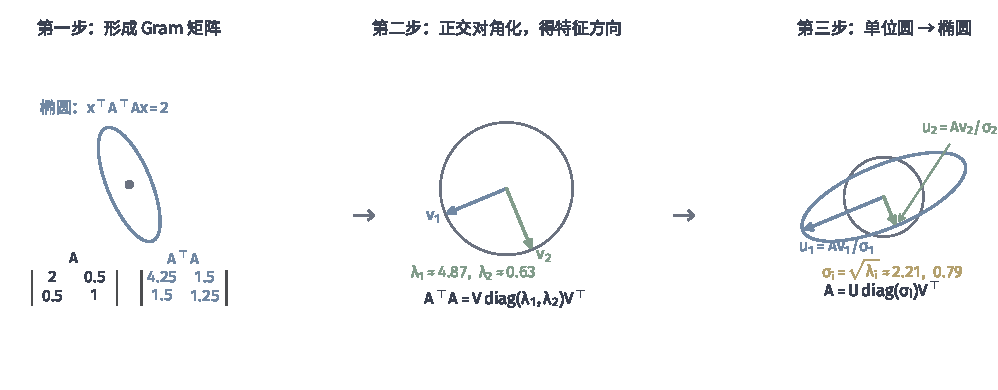
\includegraphics[width=168.998mm]{figures/00-shared/mathematical-preliminaries-upper/02-linear-spaces/matplotlib/ls-svd-construction/ls-svd-construction.pdf}
  \caption{SVD的三步构造。以$\bm A=\left[\begin{smallmatrix}2&0.5\\0.5&1\end{smallmatrix}\right]$为例：
  (1)形成$\bm A^\top\bm A=\left[\begin{smallmatrix}4.25&1.5\\1.5&1.25\end{smallmatrix}\right]$；
  (2)由谱定理对角化，特征值$\lambda_1\approx4.87,\lambda_2\approx0.63$；
  (3)$\sigma_i=\sqrt{\lambda_i}\approx2.21,0.79$，右奇异向量$\bm v_i$即特征向量，
  左奇异向量$\bm u_i=\bm A\bm v_i/\sigma_i$。解析式教学构造。}
  \label{fig:ls-svd-construction}
\end{figure*}

左奇异向量与输出端也有对称的关系。对$i\leq r$，$\bm A^\top\bm u_i=\bm A^\top\bm A\bm v_i/\sigma_i=\sigma_i\bm v_i$；对$i>r$，$\bm u_i$与$\operatorname{range}(\bm A)$正交，故对任意$\bm x$有$(\bm A^\top\bm u_i)^\top\bm x=\bm u_i^\top\bm A\bm x=0$，即$\bm A^\top\bm u_i=\bm0$。于是
\begin{equation}
 \bm A^\top\bm u_i=\sigma_i\bm v_i,\qquad
 \bm A\bm A^\top\bm u_i=\sigma_i^2\bm u_i\qquad(i\leq r),
 \label{eq:ls-svd-transpose-relation}
\end{equation}
而$i>r$时$\bm A\bm A^\top\bm u_i=\bm0$。也就是说，$\bm u_1,\ldots,\bm u_m$是$\bm A\bm A^\top$的一组标准正交特征向量，特征值依次为$\sigma_1^2,\ldots,\sigma_r^2$与$m-r$个零。$\bm A^\top\bm A$与$\bm A\bm A^\top$因而有相同的正特征值，分别在输入端与输出端给出奇异方向。

奇异值由$\bm A$唯一确定。设$\bm A=\bm U\bm\Sigma\bm V^\top$是任意一个满足定理~\ref{thm:ls-svd-existence}的分解，则$\bm A^\top\bm A=\bm V(\bm\Sigma^\top\bm\Sigma)\bm V^\top$，其中$\bm\Sigma^\top\bm\Sigma$是$d$阶对角矩阵，对角元为$\sigma_1^2,\ldots,\sigma_{\min(m,d)}^2$，$d>m$时再补$d-m$个零。$\bm V^\top=\bm V^{-1}$，所以$\bm A^\top\bm A$与$\bm\Sigma^\top\bm\Sigma$相似，由定理~\ref{thm:ls-spectrum-similarity-invariance}，二者有相同的特征多项式，$\sigma_i^2$连同重数恰是$\bm A^\top\bm A$的特征值。$\bm A^\top\bm A$只依赖$\bm A$，而$\sigma_i$是这些特征值降序排列后的非负平方根，因此与分解的选取无关：正奇异值是$\bm A^\top\bm A$正特征值的平方根，其余为零。

奇异向量则不唯一。上面的构造对$\bm A^\top\bm A$的任意一组按特征值降序排列的标准正交特征向量都成立。正奇异值重复时，对应特征空间中有许多组标准正交基可选，每选一组，再由$\bm u_i=\bm A\bm v_i/\sigma_i$确定配对的左奇异向量，都得到一个奇异值分解。把一对$\bm u_i,\bm v_i$同时变号，乘积$\sigma_i\bm u_i\bm v_i^\top$不变，两组向量仍各自标准正交，所以得到的仍是奇异值分解。

定理~\ref{thm:ls-svd-existence}中的$\bm U$、$\bm V$都是方阵，这是\emph{完整}分解，它同时给出两端的全部正交方向：$\bm v_{r+1},\ldots,\bm v_d$张成$\ker\bm A$，$\bm u_{r+1},\ldots,\bm u_m$张成$\operatorname{range}(\bm A)$的正交补。许多计算只用到前$p=\min(m,d)$列。令$\bm U_p=[\bm u_1,\ldots,\bm u_p]\in\mathbb R^{m\times p}$、$\bm V_p=[\bm v_1,\ldots,\bm v_p]\in\mathbb R^{d\times p}$、$\bm\Sigma_p=\operatorname{diag}(\sigma_1,\ldots,\sigma_p)$，则$\bm A=\bm U_p\bm\Sigma_p\bm V_p^\top$，称为经济型分解：$\bm\Sigma$中全为零的那些行或列，连同与之相乘的$\bm U$或$\bm V$的列一起删去，乘积不变。若只保留正奇异值，令$\bm U_r$、$\bm V_r$分别由前$r$个左、右奇异向量组成，$\bm\Sigma_r=\operatorname{diag}(\sigma_1,\ldots,\sigma_r)$，则
\[
 \bm A=\bm U_r\bm\Sigma_r\bm V_r^\top,\qquad
 \bm U_r\in\mathbb R^{m\times r},\ \bm\Sigma_r\in\mathbb R^{r\times r},\ \bm V_r\in\mathbb R^{d\times r},
\]
这就是和式~\eqref{eq:matrix-analysis-svd-rank-one-sum}的矩阵写法，称为秩分解形式。三种写法给出同一个矩阵，区别在于是否保留零空间方向：秩分解只描述$\bm A$真正起作用的$r$对方向，零空间与输出端正交补的基要从完整分解中读取；经济型分解在$r<p$时仍保留奇异值为零的列。

构造虽然从$\bm A^\top\bm A$出发，这条路线只用于证明存在性，并不意味着数值计算应当显式形成$\bm A^\top\bm A$。它的特征值是$\sigma_i^2$，最大与最小奇异值之比在$\bm A^\top\bm A$中变成平方，小奇异值相对于大奇异值变得更小；第~\ref{sec:ls-ls-regularization-sensitivity}节以最小二乘的正规方程为例，分析这种平方带来的误差风险。实际计算奇异值分解的算法直接作用于$\bm A$本身，其构造与误差分析不在本书展开。

\subsection{奇异值与矩阵的大小}
\label{sec:ls-svd-matrix-size}

几何上，SVD把$\bm A$的作用拆成三步：$\bm V^\top$把输入写成右奇异方向上的坐标，$\bm\Sigma$把第$i$个坐标乘以$\sigma_i$，$\bm U$再把结果放到输出空间的左奇异方向上。正交矩阵保持长度，所以只有中间一步改变长度。于是$\bm A$把输入端的单位球映成输出空间中一个椭球（秩亏时它落在低维子空间内）。具体地，单位球中的$\bm x=\sum_ic_i\bm v_i$满足$\sum_ic_i^2\leq1$，其像为$\bm y=\sum_{i\leq r}\sigma_ic_i\bm u_i$，它落在$\operatorname{span}\{\bm u_1,\ldots,\bm u_r\}$中，坐标$y_i=\bm u_i^\top\bm y=\sigma_ic_i$满足$\sum_{i\leq r}(y_i/\sigma_i)^2=\sum_{i\leq r}c_i^2\leq1$；反过来，该子空间中满足这一不等式的$\bm y$是$\bm x=\sum_{i\leq r}(y_i/\sigma_i)\bm v_i$的像，而这个$\bm x$在单位球中。所以像恰为
\[
 \Bigl\{\bm y\in\operatorname{span}\{\bm u_1,\ldots,\bm u_r\}:\ \sum_{i=1}^r\frac{(\bm u_i^\top\bm y)^2}{\sigma_i^2}\leq1\Bigr\},
\]
即以$\sigma_i\bm u_i$为半轴的椭球：$\bm v_i$方向的单位向量被送到半轴端点$\sigma_i\bm u_i$。若$r<d$，单位球面上的点也可能映到这个椭球的内部，例如$(\bm v_1+\bm v_d)/\sqrt2$被送到$\sigma_1\bm u_1/\sqrt2$，所以这里用单位球而不是球面描述整个像。图~\ref{fig:matrix-analysis-svd-geometry}用二维旋转矩阵$\bm R(\theta)=\left[\begin{smallmatrix}\cos\theta&-\sin\theta\\\sin\theta&\cos\theta\end{smallmatrix}\right]$构造了一个输入方向与输出方向不同的例子。

\begin{figure*}[htbp]
  \centering
  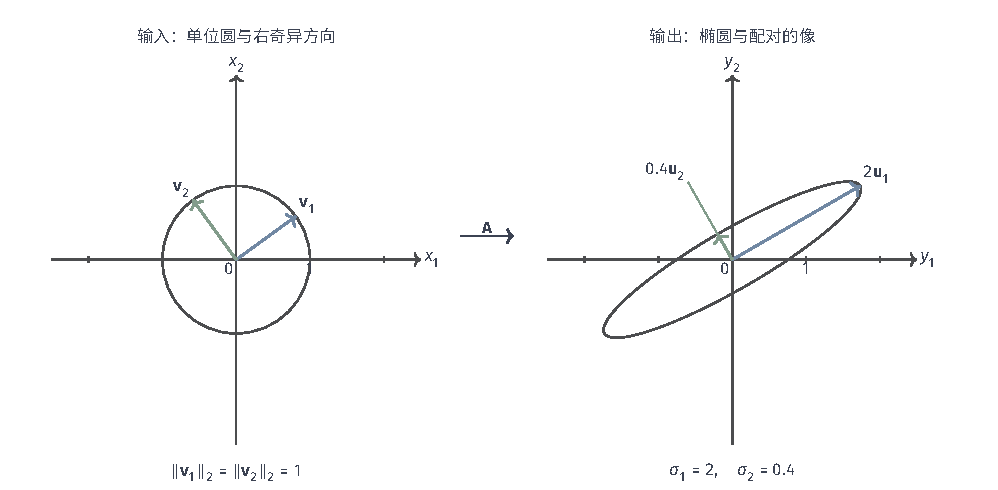
\includegraphics[width=168.998mm]{figures/00-shared/mathematical-preliminaries-upper/02-linear-spaces/tikz/matrix-analysis-svd-geometry/figure.pdf}
  \caption{矩阵$\bm A=\bm R(\pi/6)\operatorname{diag}(2,0.4)\bm R(\pi/5)^\top$
  将单位圆变为椭圆。蓝、绿分别对应两个奇异方向；同色箭头在左侧标出$\bm v_i$，
  在右侧标出其像$\sigma_i\bm u_i$。两侧坐标比例相同。奇异值决定长度变化，左右方向可以不同，
  因而这不是沿特征方向的同空间缩放。图为教学构造。}
  \label{fig:matrix-analysis-svd-geometry}
\end{figure*}

第~\ref{sec:ls-frobenius-norm}节与第~\ref{sec:ls-matrix-norms}节分别定义了Frobenius范数与谱范数，但没有给出谱范数的算法。按上面的三步读法，椭球的最长半轴就是最强的放大，各半轴长度的平方和就是全部伸缩的总量。对$\bm x=\sum_ic_i\bm v_i$，由$\bm u_i$标准正交，
\[
 \lVert\bm A\bm x\rVert_2^2=\sum_{i\leq r}\sigma_i^2c_i^2\leq\sigma_1^2\sum_ic_i^2=\sigma_1^2\lVert\bm x\rVert_2^2 ,
\]
等号在$\bm x=\bm v_1$时成立；而由$\bm A^\top\bm A=\bm V(\bm\Sigma^\top\bm\Sigma)\bm V^\top$与迹的循环性，$\lVert\bm A\rVert_{\mathrm F}^2=\operatorname{tr}(\bm A^\top\bm A)=\operatorname{tr}(\bm\Sigma^\top\bm\Sigma\bm V^\top\bm V)=\sum_i\sigma_i^2$。因此
\begin{align}
 \lVert\bm A\rVert_2&=\sigma_1,
 \label{eq:matrix-analysis-spectral-norm}\\
 \lVert\bm A\rVert_{\mathrm F}&=\Bigl(\sum_{i=1}^r\sigma_i^2\Bigr)^{1/2}.
 \label{eq:matrix-analysis-frobenius-norm}
\end{align}
正奇异值的个数等于$\operatorname{rank}\bm A$，这已在构造中证明。

同一展开也给出最弱的放大倍数，但要先区分零空间。$\ker\bm A$中的非零输入被送到零，它们的输出长度不提供信息；有意义的问题是在$\ker\bm A$的正交补$\operatorname{span}\{\bm v_1,\ldots,\bm v_r\}$上，单位输入至少被送出多远。满列秩时$\ker\bm A=\{\bm0\}$，这个正交补就是整个输入空间。最后，可逆方阵的逆矩阵把每个伸缩倍数倒过来，最弱的放大变成逆矩阵最强的放大。下面的定理汇总这几项读数。

\begin{theorem}[最小奇异值与逆矩阵的范数]
\label{thm:ls-svd-singular-value-norms}
设$\bm A\in\mathbb R^{m\times d}$的秩为$r\geq1$，奇异值分解如定理~\ref{thm:ls-svd-existence}所示。
\begin{enumerate}
 \item 对$\ker\bm A$的正交补中的任意$\bm x$，$\lVert\bm A\bm x\rVert_2\geq\sigma_r\lVert\bm x\rVert_2$，等号在$\bm x=\bm v_r$时成立。
 \item 若$\bm A$满列秩，即$r=d\leq m$，则对所有$\bm x\in\mathbb R^d$，$\lVert\bm A\bm x\rVert_2\geq\sigma_d\lVert\bm x\rVert_2$，且
 \[
  \min_{\lVert\bm x\rVert_2=1}\lVert\bm A\bm x\rVert_2=\sigma_d>0 .
 \]
 \item 若$\bm A$是可逆方阵（$m=d=r$），则$\bm A^{-1}=\sum_{i=1}^d\sigma_i^{-1}\bm v_i\bm u_i^\top$，并且
 \begin{equation}
  \lVert\bm A^{-1}\rVert_2=\frac1{\sigma_d}.
  \label{eq:ls-svd-inverse-norm}
 \end{equation}
\end{enumerate}
\end{theorem}
\begin{proof}
由构造，$\ker\bm A$由$\bm v_{r+1},\ldots,\bm v_d$张成，其正交补由$\bm v_1,\ldots,\bm v_r$张成。对其中的$\bm x=\sum_{i\leq r}c_i\bm v_i$，
\[
 \lVert\bm A\bm x\rVert_2^2=\sum_{i\leq r}\sigma_i^2c_i^2\geq\sigma_r^2\sum_{i\leq r}c_i^2=\sigma_r^2\lVert\bm x\rVert_2^2 ,
\]
其中用到$\sigma_i\geq\sigma_r$（$i\leq r$）；取$\bm x=\bm v_r$时只有$c_r=1$，等号成立。这是第一条。满列秩时正交补就是$\mathbb R^d$，且$\sigma_r=\sigma_d>0$，第一条即给出第二条。

对第三条，令$\bm B=\sum_i\sigma_i^{-1}\bm v_i\bm u_i^\top$。由$\bm v_i^\top\bm v_j=\delta_{i,j}$，
\[
 \bm A\bm B=\sum_{i,j}\sigma_i\sigma_j^{-1}\bm u_i(\bm v_i^\top\bm v_j)\bm u_j^\top=\sum_i\bm u_i\bm u_i^\top=\bm U\bm U^\top=\bm I,
\]
方阵的右逆就是逆，所以$\bm B=\bm A^{-1}$。这个和式本身就是$\bm A^{-1}$的奇异值分解：右奇异向量为$\bm u_i$，左奇异向量为$\bm v_i$，奇异值为$\sigma_i^{-1}$，其中最大的是$\sigma_d^{-1}$。由式~\eqref{eq:matrix-analysis-spectral-norm}，$\lVert\bm A^{-1}\rVert_2=1/\sigma_d$。
\end{proof}

满列秩只保证最小放大倍数为正，并不保证它不太小。式~\eqref{eq:ls-svd-inverse-norm}说明，最小奇异值越小，逆矩阵把输出端的误差放大得越厉害；最大奇异值衡量最强的放大，最小奇异值衡量最弱的放大，二者之比就是第~\ref{sec:ls-matrix-condition-number}节的矩阵条件数，它决定线性方程的解对数据误差有多敏感。当$r<d$时（$m<d$时总是如此），存在非零输入被送到零，单位输入的最小输出长度为零，这时只能在零空间的正交补上谈最弱的放大。最弱放大的方向$\bm v_d$也有直接用处：第~\ref{sec:linear-algebra-homogeneous-estimation}节的齐次最小二乘在单位向量中最小化$\lVert\bm A\bm x\rVert_2$，最优解就是$\bm v_d$。

至此，本章的表示问题有了回答。由特征向量组成的基（若存在）使算子的矩阵成为对角形；要求基标准正交时，对称矩阵仍能对角化，一般方阵只能化为实Schur形；输入、输出各取一组标准正交基时，任意矩阵都能化为对角形。下一节转向第一个具体问题：固定对称矩阵，在长度约束下比较二次型的大小。
